\documentclass[12pt]{article}
\usepackage[utf8]{inputenc}
\usepackage[spanish]{babel}
\usepackage[all]{xy}
\usepackage{amsfonts, amssymb, amsmath, mathrsfs}
\usepackage{anysize}
\usepackage{graphicx}
\usepackage{caption}
\usepackage{subcaption}
\usepackage[dvipsnames, x11names]{xcolor}
\usepackage{otros/pgf-pie}
\usepackage{tikz}
\usetikzlibrary{positioning}
\usetikzlibrary{decorations.pathmorphing, patterns,shapes, arrows}
\usepackage{pgfplots}
\pgfplotsset{compat=1.12}
\PassOptionsToPackage{demo}{graphicx}




\renewcommand{\baselinestretch}{1}
\setlength{\parskip}{\baselineskip}


\def\Put(#1,#2)#3{\leavevmode\makebox(0,0){\put(#1,#2){#3}}}

\definecolor{colorClase}{rgb}{0.82,0.565,0}




\begin{document}
\listoffigures

\vfill
{\color{Magenta4}\rule{\linewidth}{3mm}}
\vfill
{\color{Seashell4!60!SlateBlue4!}\rule{\linewidth}{3mm}}
\vfill
{\color{blue!20!red!40!}\rule{\linewidth}{3mm}}
\vfill
{\color{Tomato1}\rule{\linewidth}{3mm}}
\vfill
{\color{Firebrick1}\rule{\linewidth}{3mm}}
\vfill
{\color{Firebrick4!50!DeepPink1!90!}\rule{\linewidth}{3mm}}
\vfill
{\color[rgb]{0.169,0, 0.6}\rule{\linewidth}{3mm}}



\newpage
\begin{figure}
    \centering
    \begin{subfigure}{0.49\linewidth}
    \centering
    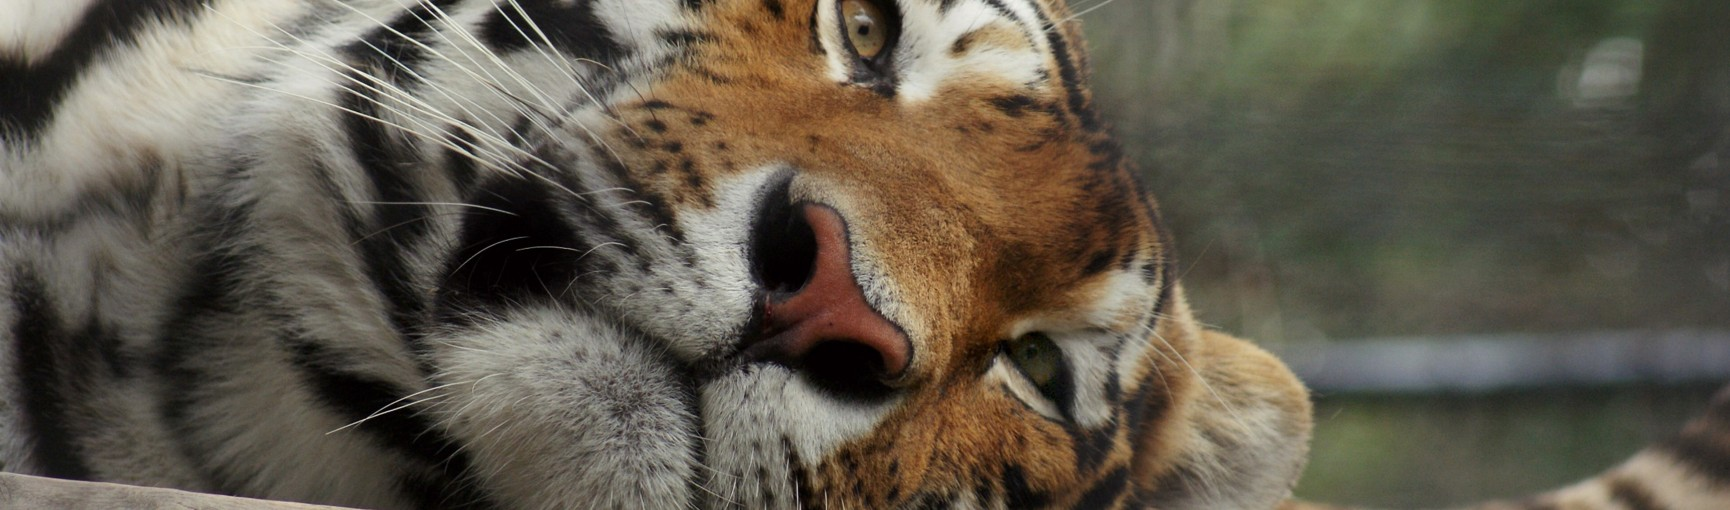
\includegraphics[width=0.7\linewidth]{animals/animal1.jpeg}
    \caption{Animal 1}
    \label{fig:animal1}
    \end{subfigure}
    \begin{subfigure}{0.49\linewidth}
    \centering
    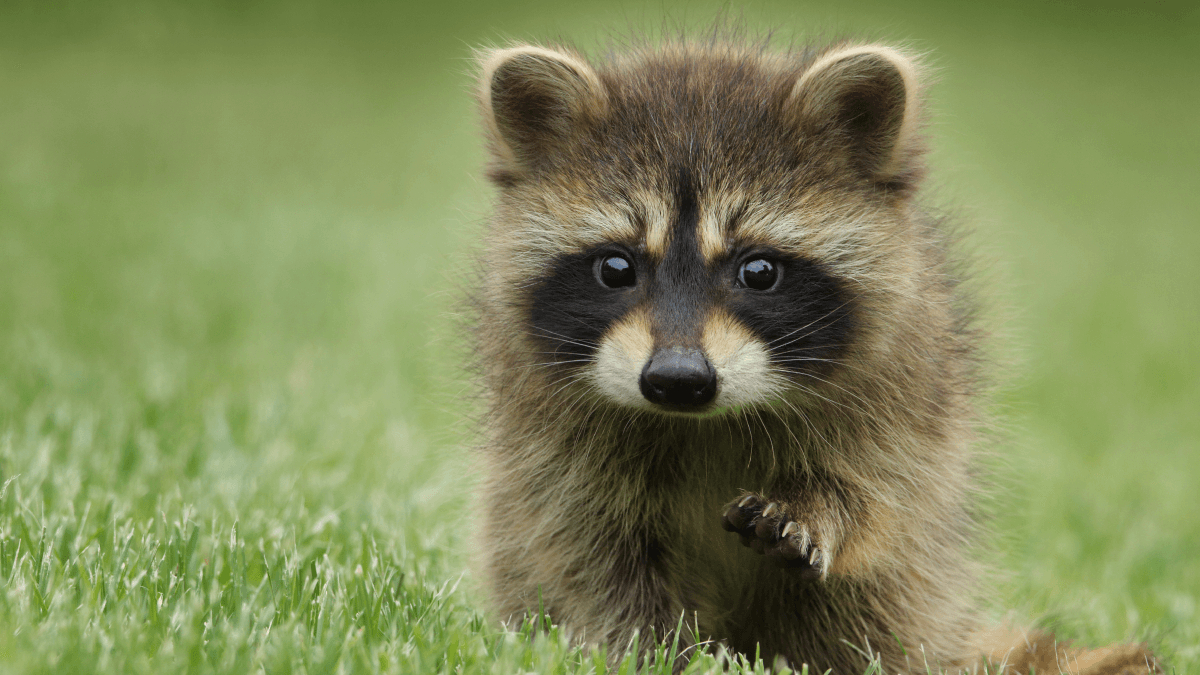
\includegraphics[width=0.7\linewidth]{animals/animal2.png}
    \caption{Animal 2}
    \label{fig:animal2}
    \end{subfigure}
    \begin{subfigure}{0.49\linewidth}
    \centering
    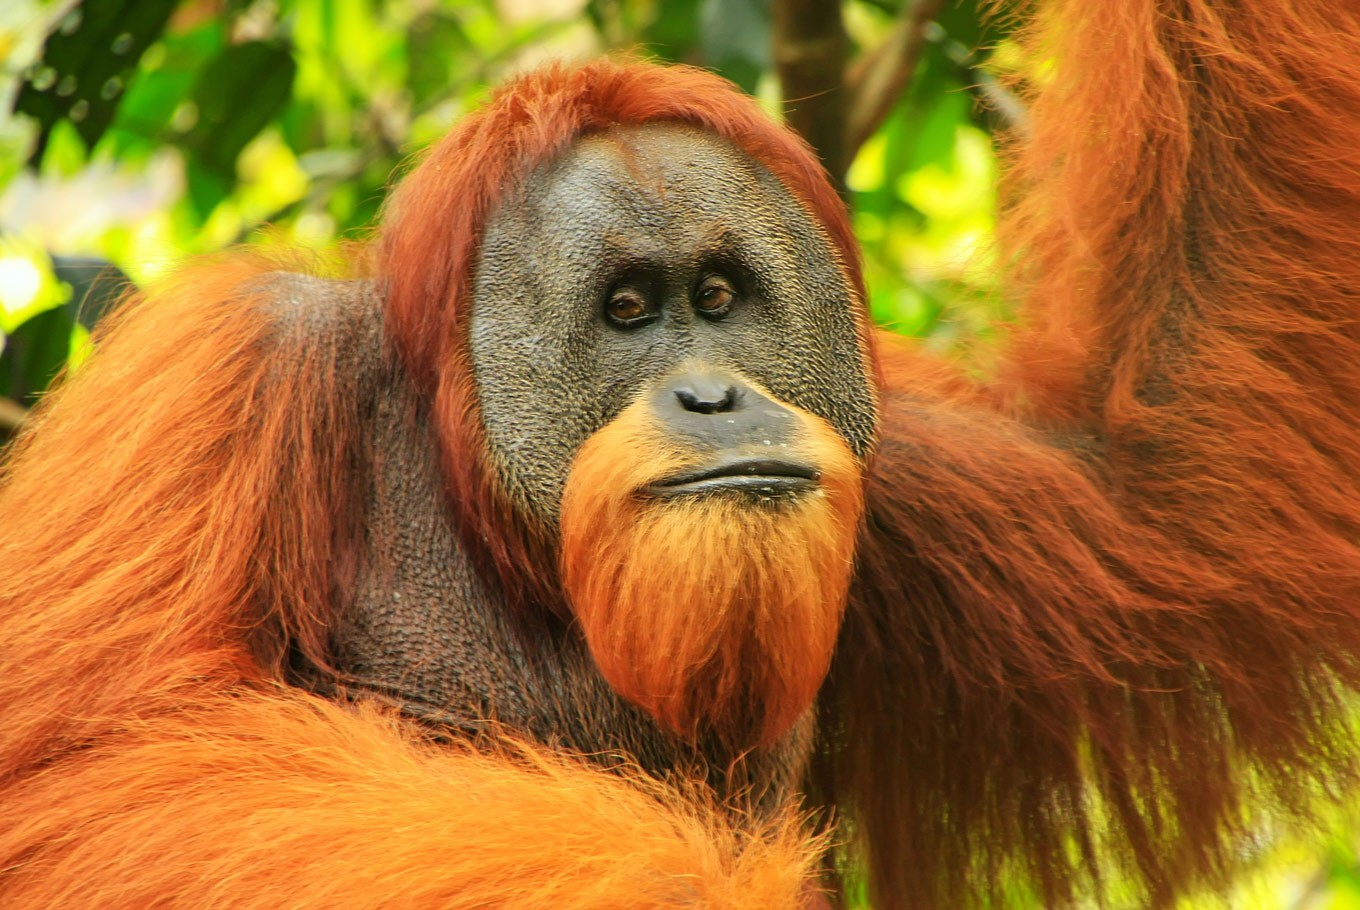
\includegraphics[width=0.7\linewidth]{animals/animal3.jpg}
    \caption{Animal 3}
    \label{fig:animal3}
    \end{subfigure}
    \begin{subfigure}{0.49\linewidth}
    \centering
    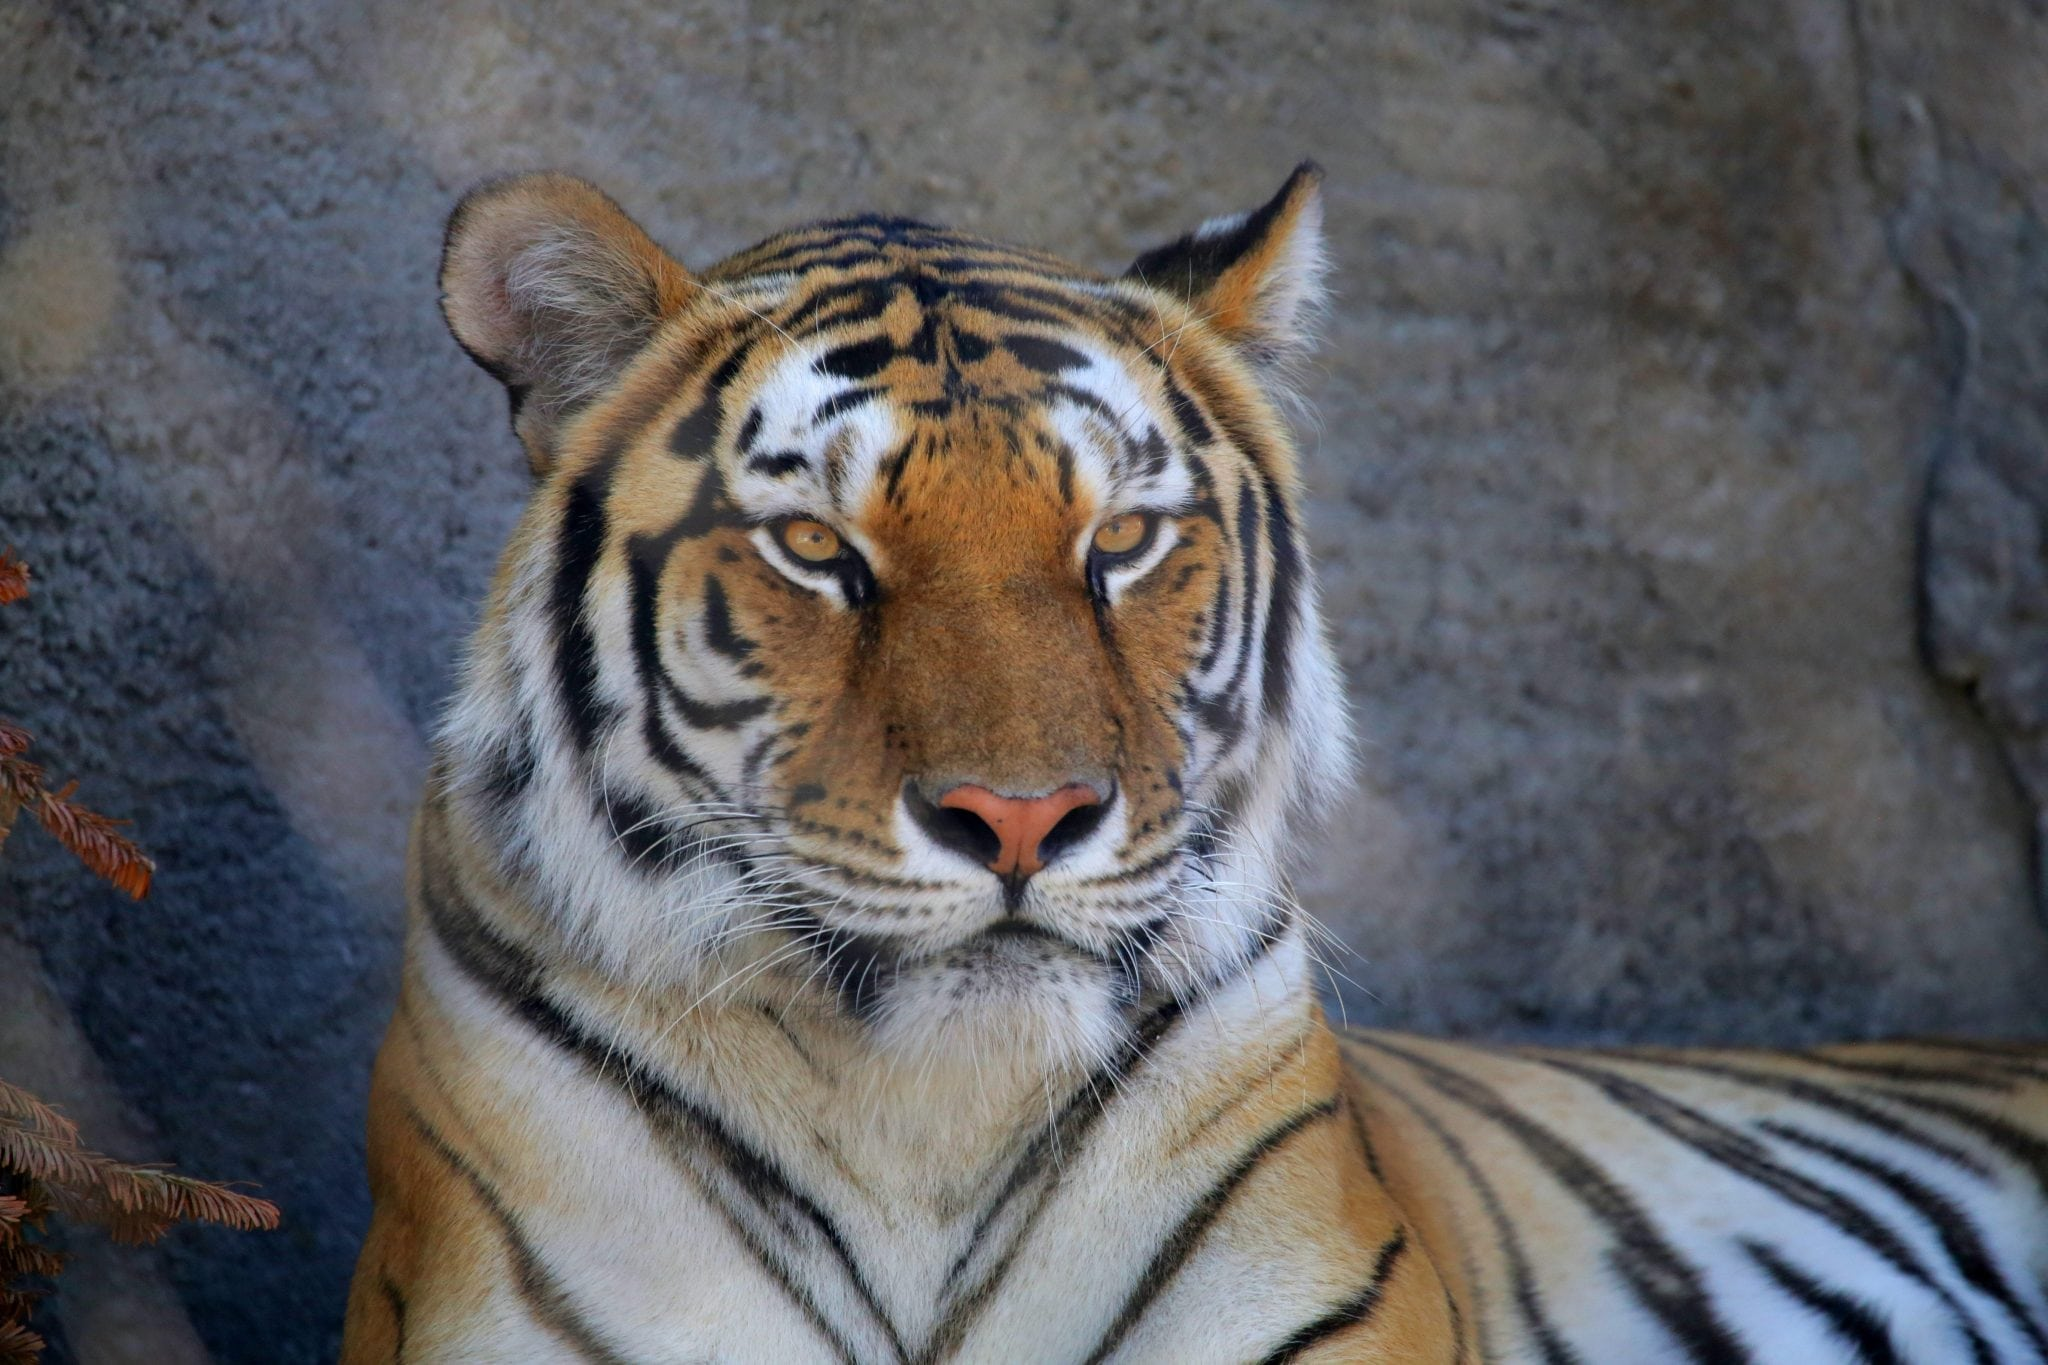
\includegraphics[width=0.7\linewidth]{animals/animal4.jpg}
    \caption{Animal 4}
    \label{fig:animal4}
    \end{subfigure}
    \begin{subfigure}{0.49\linewidth}
    \centering
    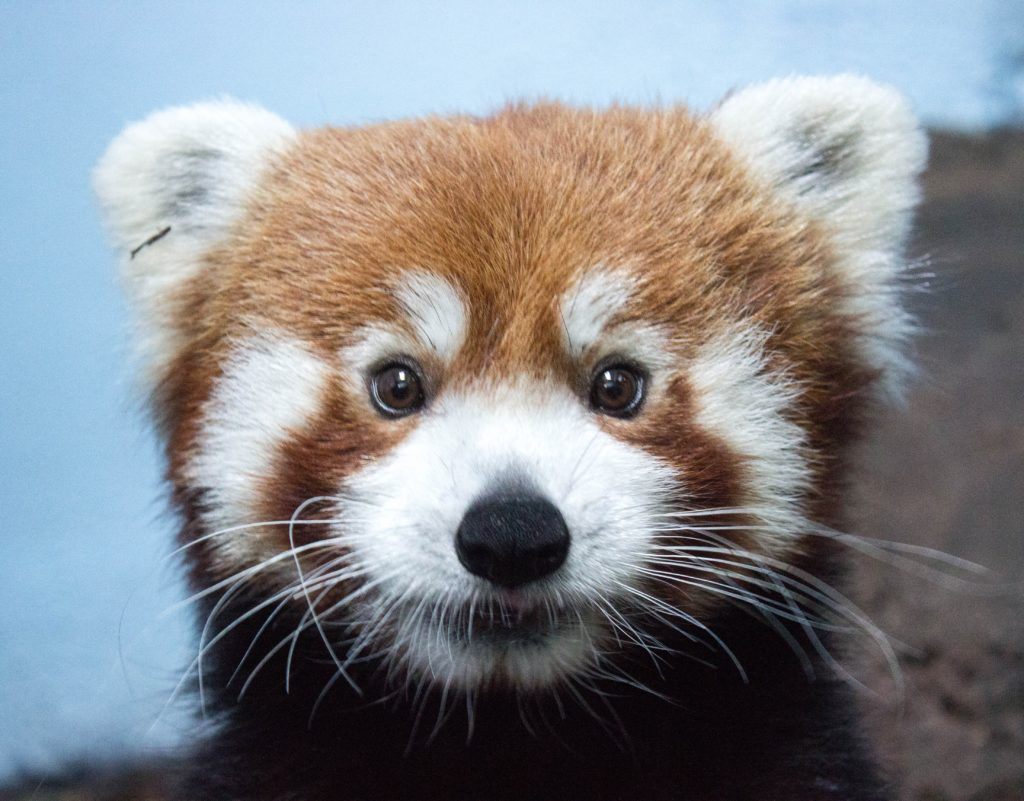
\includegraphics[width=0.7\linewidth]{animals/animal5.jpg}
    \caption{Animal 5}
    \label{fig:animal5}
    \end{subfigure}
    \begin{subfigure}{0.49\linewidth}
    \centering
    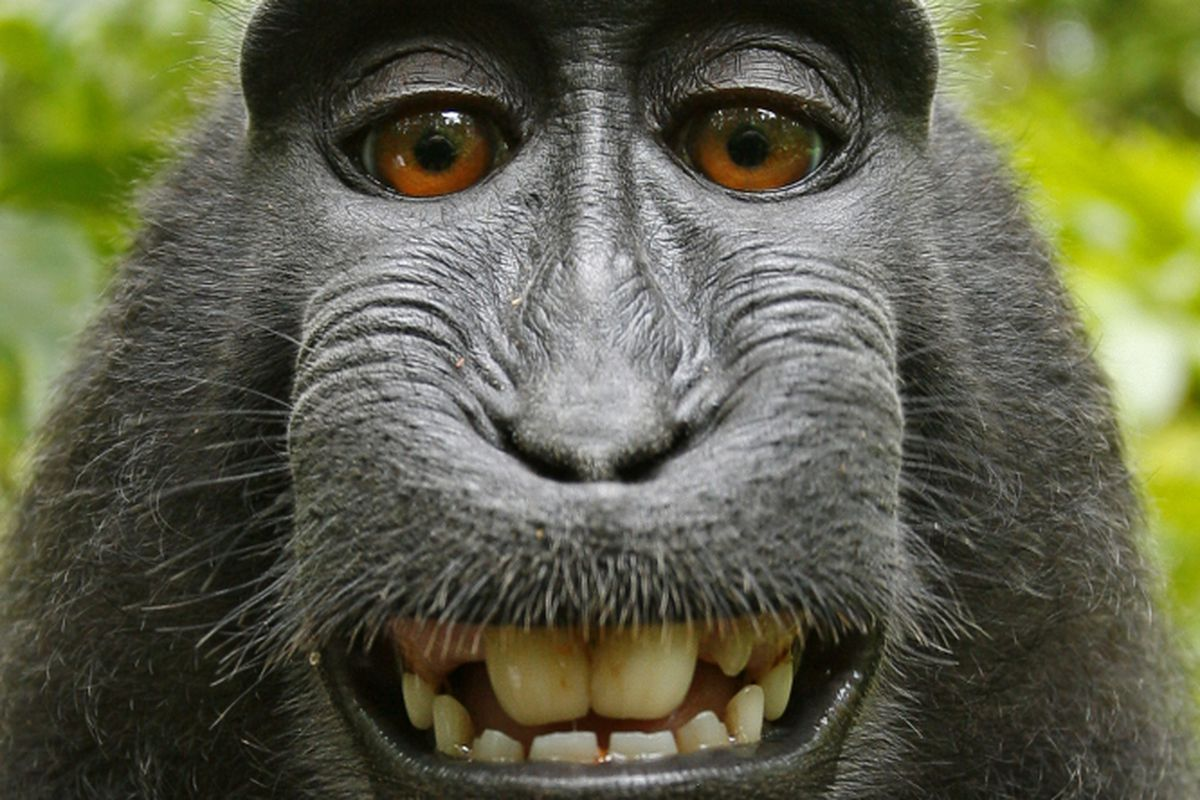
\includegraphics[width=0.7\linewidth]{animals/animal6.jpg}
    \caption{Animal 6}
    \label{fig:animal6}
    \end{subfigure}
    \begin{subfigure}{0.49\linewidth}
    \centering
    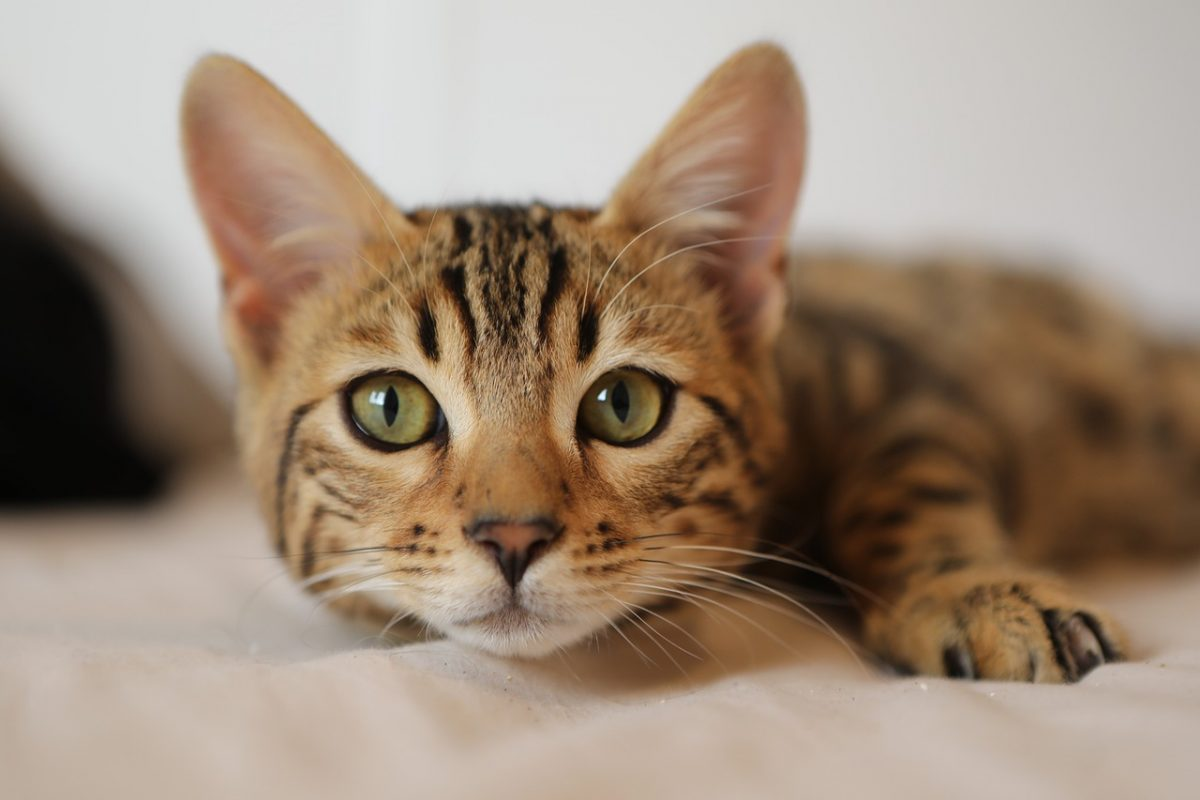
\includegraphics[width=0.7\linewidth]{animals/animal7.jpg}
    \caption{Animal 7}
    \label{fig:animal7}
    \end{subfigure}
    \begin{subfigure}{0.49\linewidth}
    \centering
    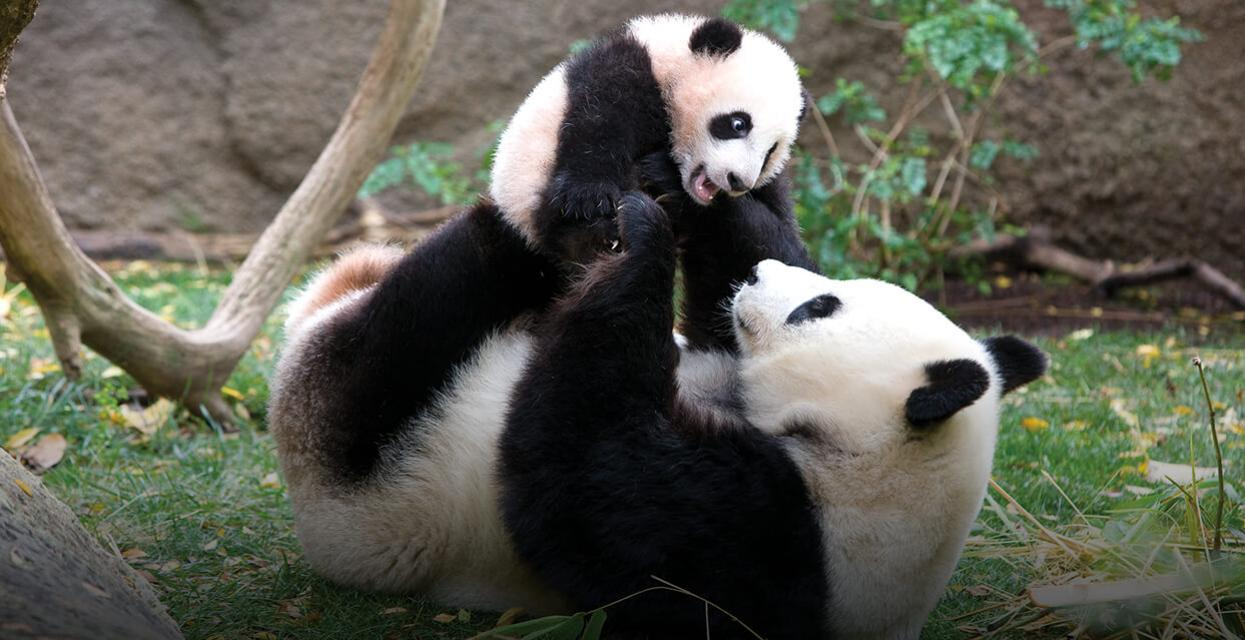
\includegraphics[width=0.7\linewidth]{animals/animal8.jpg}
    \caption{Animal 8}
    \label{fig:animal8}
    \end{subfigure}
    \begin{subfigure}{0.49\linewidth}
    \centering
    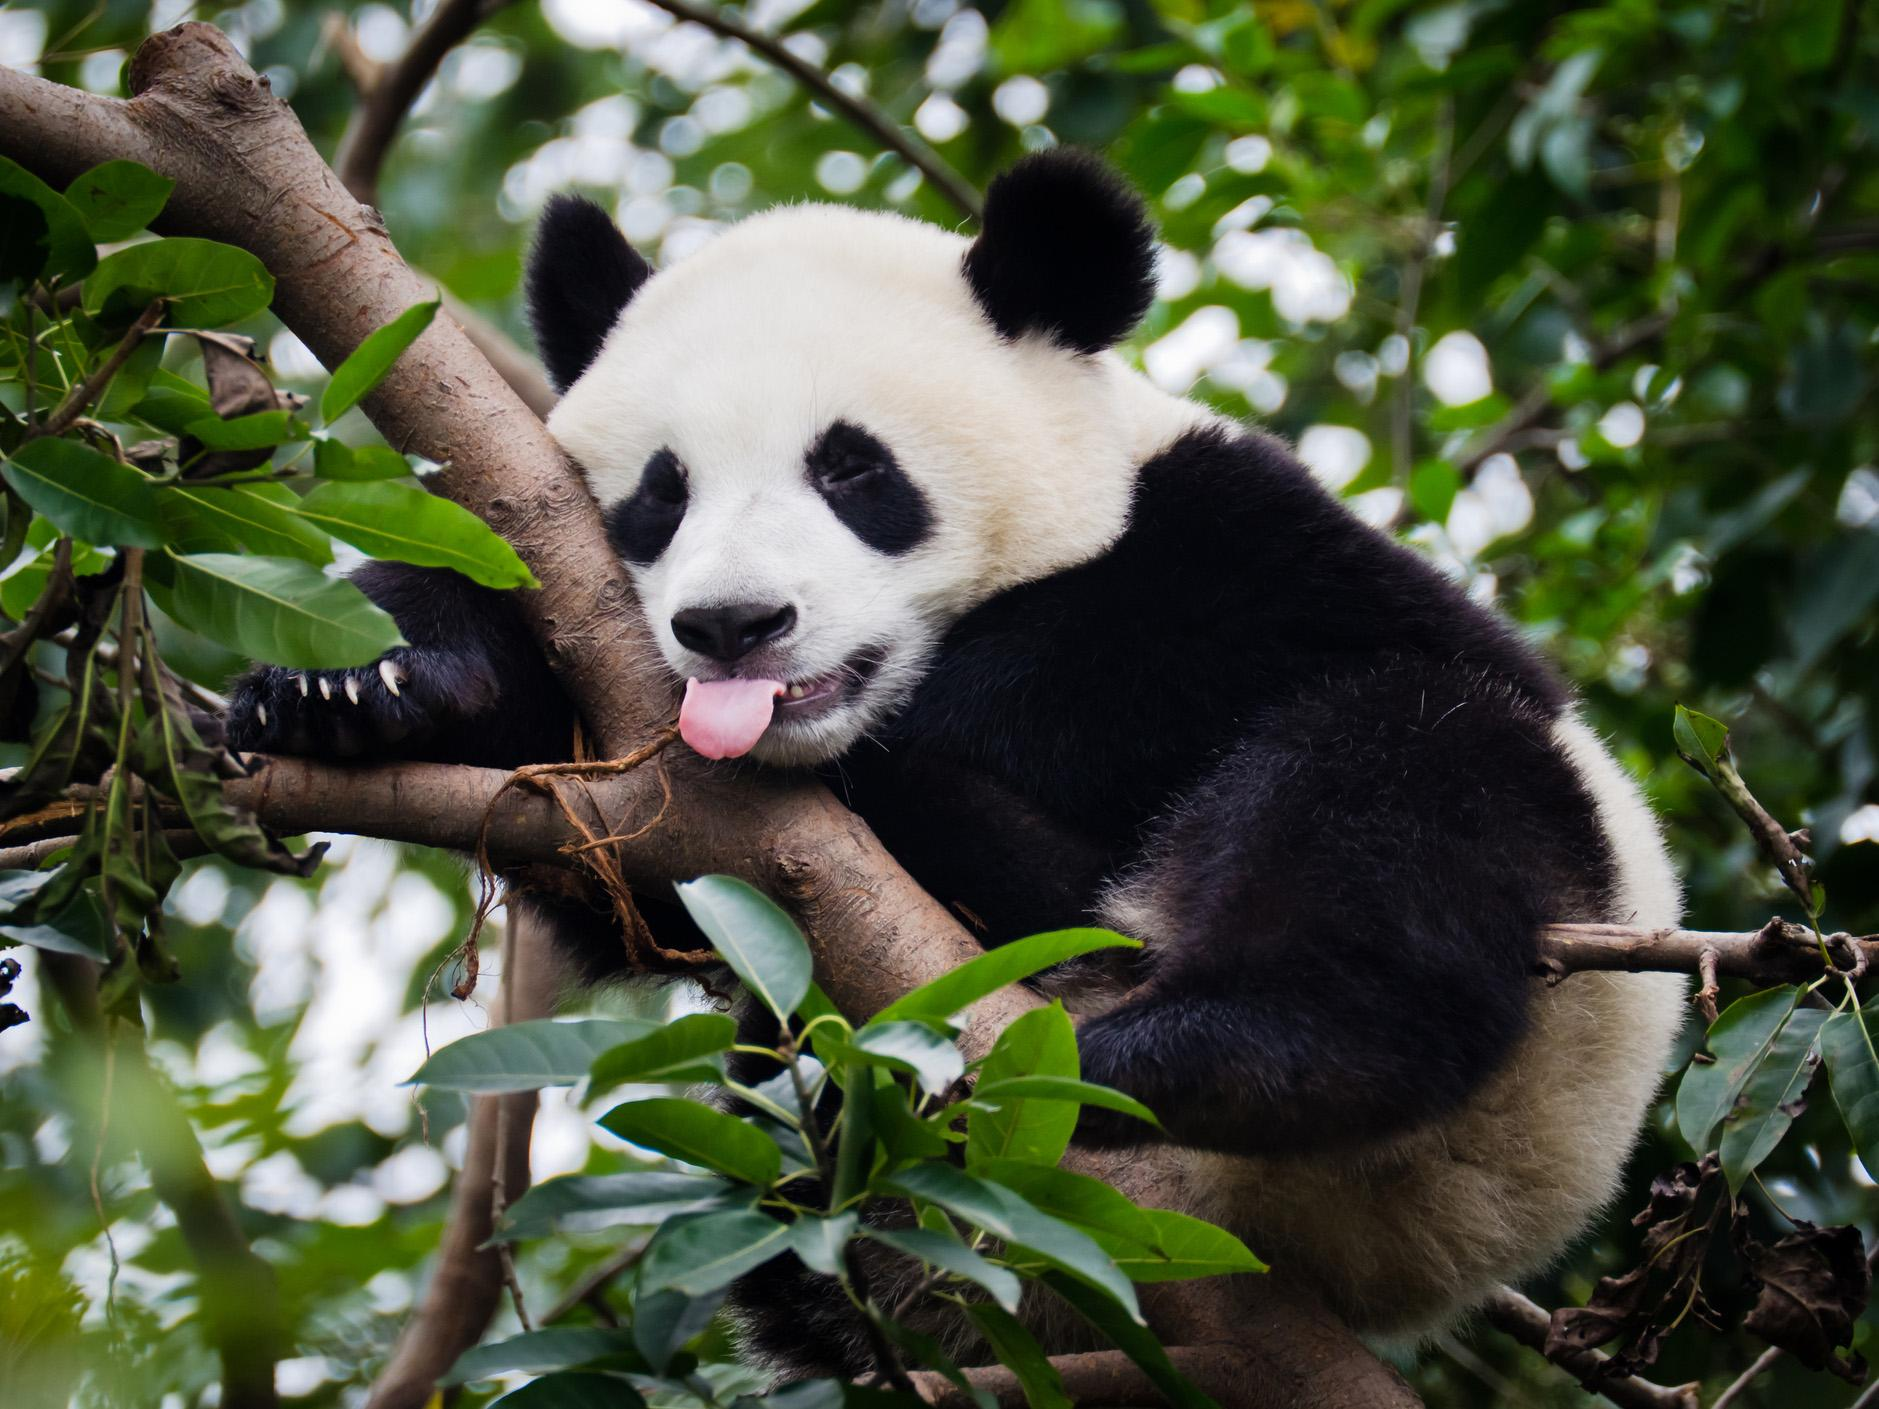
\includegraphics[width=0.7\linewidth]{animals/animal9.jpg}
    \caption{Animal 9}
    \label{fig:animal9}
    \end{subfigure}
    \caption{Animales}
\end{figure}
\newpage
\begin{figure}[h!]
    \centering
    \begin{tikzpicture}
    \node[fill=Seashell4!80, circle](A){A};
     \node[fill= LightGoldenrod1, ellipse] (B) [above right = 1cm and 1.5cm of A] {B};
    \node[fill= Tomato1, ellipse] (C) [below right = 0.6cm and 2cm of A] {C};
      \node[fill=  SteelBlue1, ellipse] (D) [above left = 1cm and 1.5cm of A] {D};
      \node[fill= Turquoise, ellipse] (E) [below left = 0.6cm and 2cm of A] {E};
      \node[fill= MediumPurple1 , ellipse] (F) [below = 1.2cm of A] {F};
      
      \path[every node/.style={font=\sffamily\small}]
      (A) edge (B)
        edge[thick, dashed] (C)
    edge[ thick, dashed] (D)
    edge[ thick, dashed] (E)
    edge[ thick, dashed] (F)
    (B) edge[ thick, dashed, bend left] (C);
\end{tikzpicture}
    \caption{Nodos y caminos}
    \label{fig:tikz1}
\end{figure}

\begin{figure}
    \centering
    \begin{tikzpicture}
\pie[cloud, text=pin, scale font]
{10/A,23/B, 5/C,10/D, 12/E,17/F, 20/G, 3/H}
\end{tikzpicture}
    \caption{Nubes}
    \label{fig:tikz2}
\end{figure}

\end{document}